\documentclass[11pt,a4paper]{article}
\usepackage[utf8]{inputenc}
\usepackage{amsmath,amsfonts,amssymb}
\usepackage{graphicx}
\usepackage{geometry}
\geometry{margin=1in}
\usepackage{booktabs}
\usepackage{hyperref}
\usepackage{float}
\usepackage{xcolor}

\title{\textbf{EE3621: Digital Signal Processing} \\ \Large Lecture 16: Adaptive Filtering --- LMS Algorithm \\ \large (III B.Tech EEE)}
\author{Lecture Notes (40-Minute Plan)}
\date{}

\definecolor{darkbg}{HTML}{0d121f}
\definecolor{lighttext}{HTML}{e2e8f0}
\definecolor{primary}{HTML}{8b5cf6}
\definecolor{secondary}{HTML}{0dd5c5}

\pagecolor{darkbg}
\color{lighttext}

\hypersetup{
    colorlinks=true,
    linkcolor=secondary,
    urlcolor=secondary
}

\begin{document}

\maketitle

\section{Lecture Plan \& Objectives (40 Minutes Breakdown)}
\begin{itemize}
    \item \textbf{00:00 -- 05:00 (5 mins):} Intro to Adaptive Filtering, non-stationary environments, and limits of static Wiener filters.
    \item \textbf{05:00 -- 12:00 (7 mins):} Steepest Descent Algorithm, MSE cost function $J(\mathbf{w})$, exact gradient, eigenvalue spread.
    \item \textbf{12:00 -- 20:00 (8 mins):} LMS Algorithm Derivation, instantaneous gradient $\hat{\nabla} J$, error $e[n]$, and weight update rule.
    \item \textbf{20:00 -- 25:00 (5 mins):} Convergence conditions ($\mu < 1/\lambda_{\max}$) and time constant $\tau_k$.
    \item \textbf{25:00 -- 30:00 (5 mins):} Misadjustment $M$ and Normalized LMS (NLMS).
    \item \textbf{30:00 -- 33:00 (3 mins):} RLS Algorithm outline.
    \item \textbf{33:00 -- 40:00 (7 mins):} Real-world Applications (Acoustic Echo Cancellation) and Checkpoint questions.
\end{itemize}

\noindent\rule{\textwidth}{0.5pt}

\section{Why Adaptive Filtering?}
Classical digital signal processing often assumes that signals are stationary and their statistics (like autocorrelation) are perfectly known. If known, an optimal Wiener filter can be designed. However, in practice:
\begin{enumerate}
    \item \textbf{Non-stationary environments:} Signal statistics vary over time.
    \item \textbf{Unknown statistics:} We often lack prior knowledge of the channel or interference.
    \item \textbf{Real-time constraints:} Computing and inverting large autocorrelation matrices in real-time is computationally unfeasible.
\end{enumerate}
Adaptive filters dynamically adjust their coefficients to track changing environments. A standard FIR architecture is commonly utilized, as shown below for reference.

\section{Steepest Descent Algorithm}

\begin{figure}[H]
    \centering
    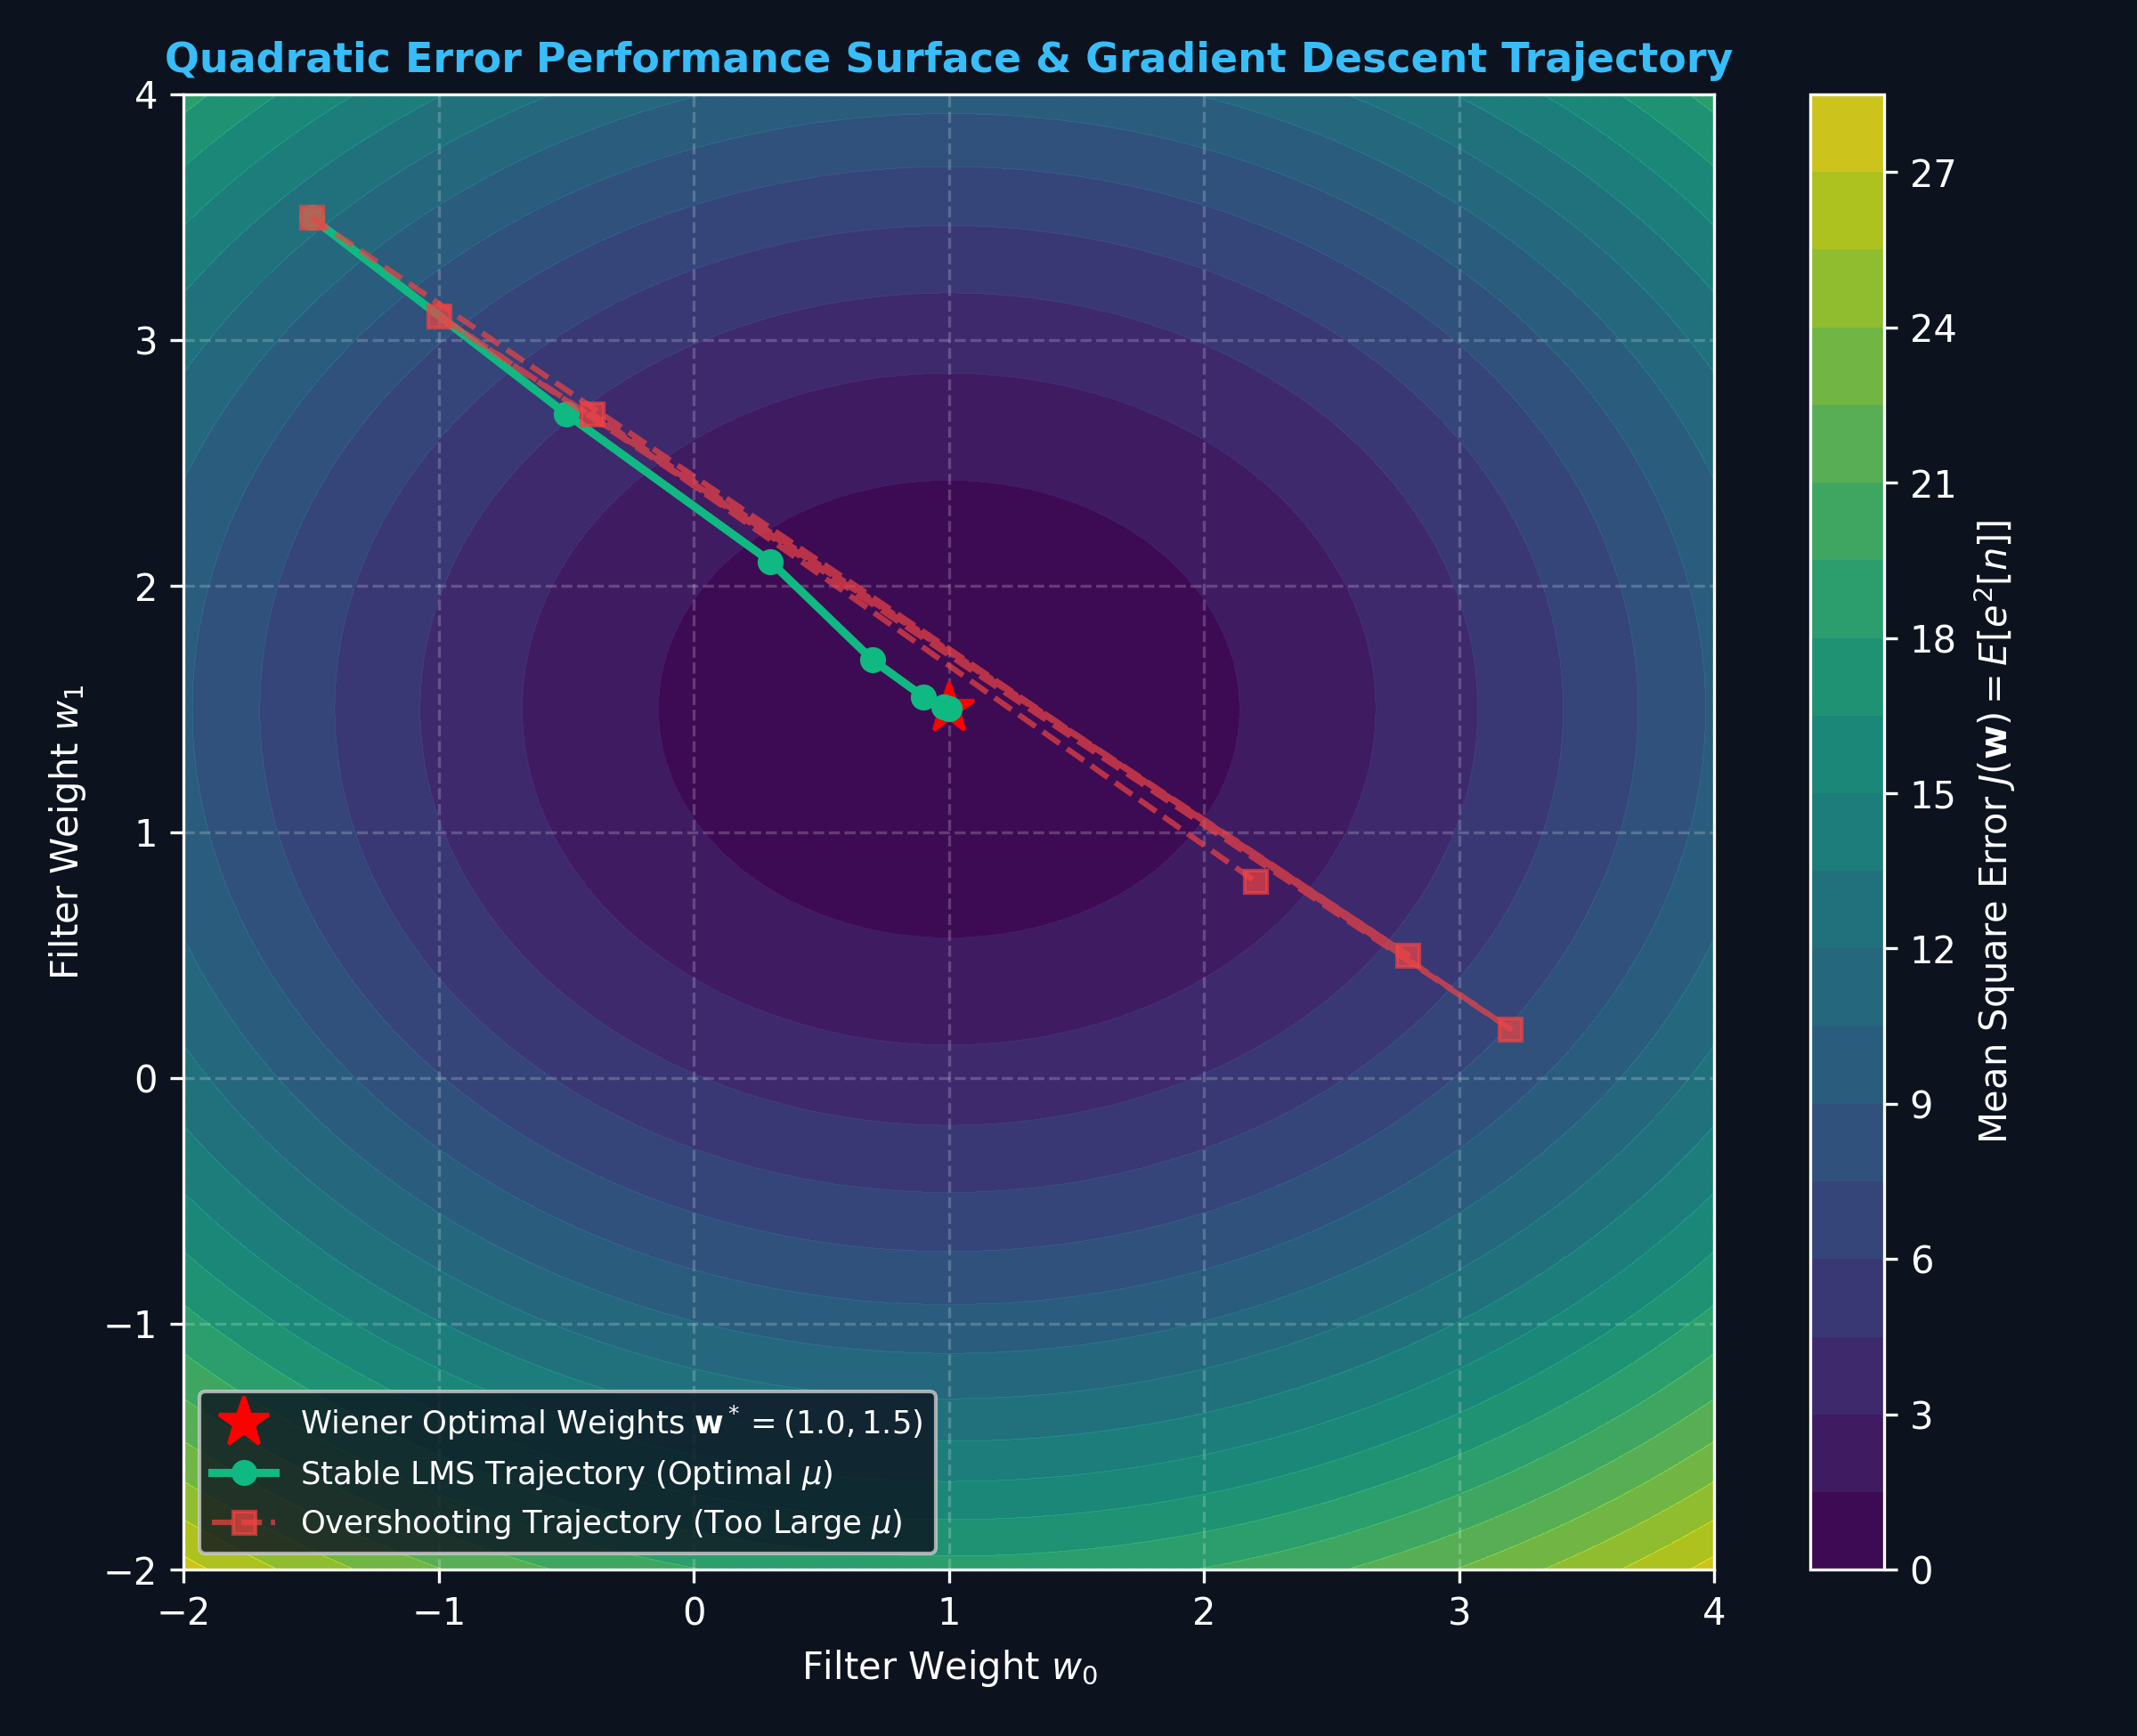
\includegraphics[width=0.75\textwidth]{images/lms_error_performance_surface.png}
    \caption{Quadratic MSE Error Performance Surface and Stochastic Gradient Descent Trajectory.}
\end{figure}

\begin{figure}[H]
    \centering
    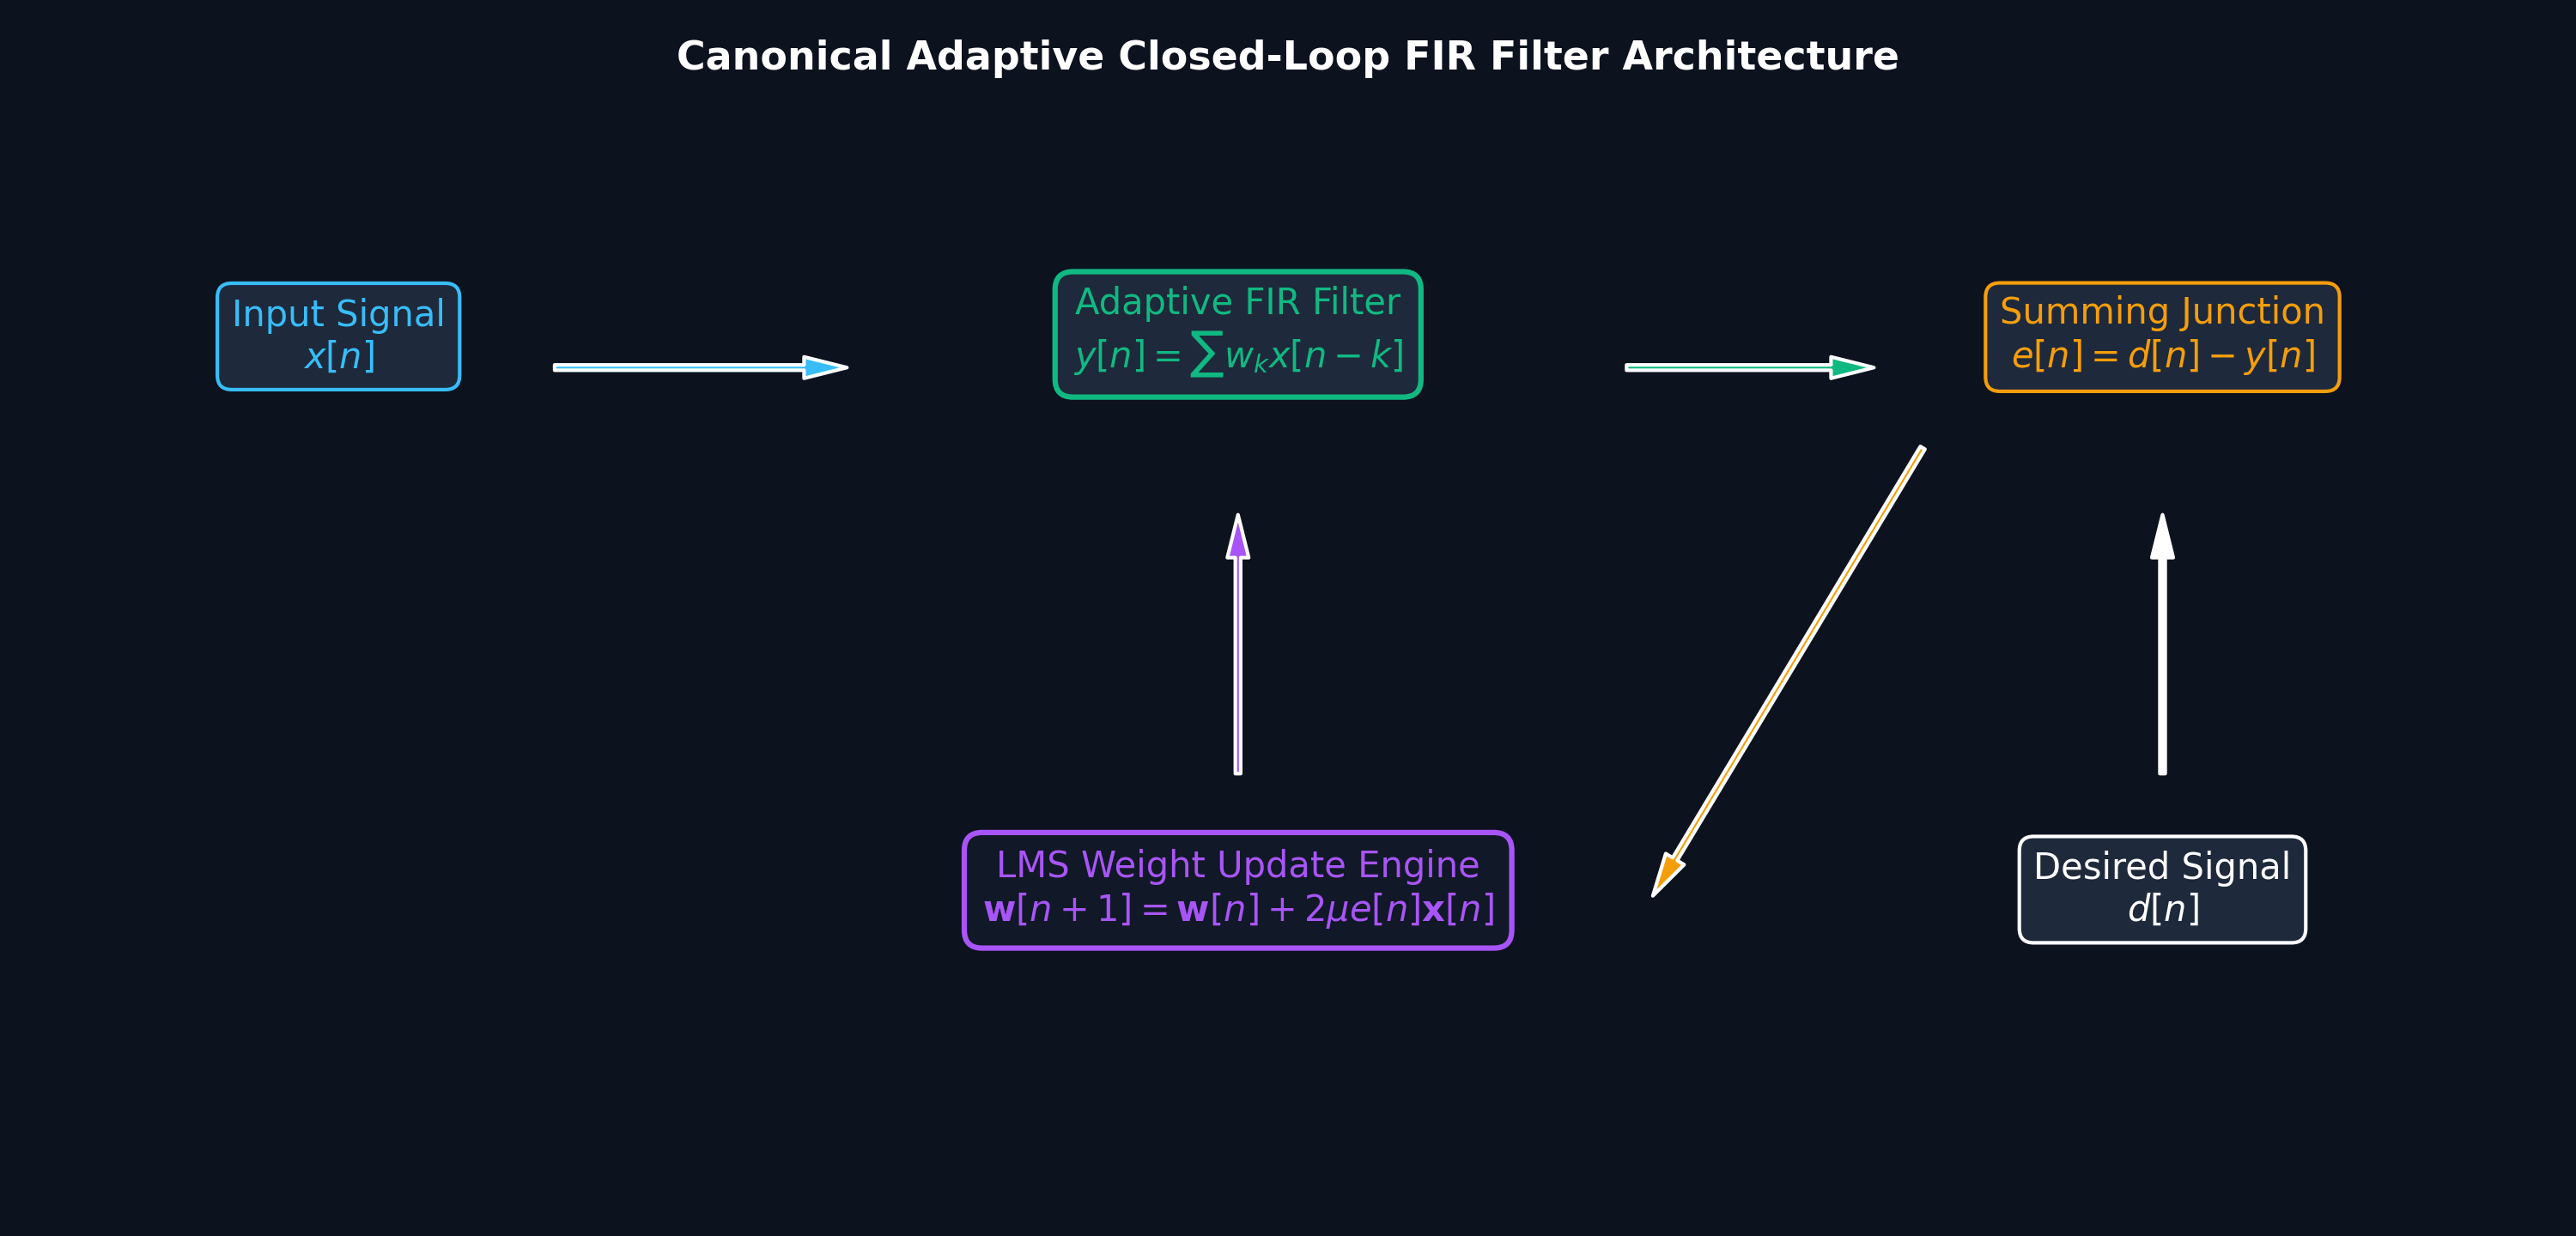
\includegraphics[width=0.85\textwidth]{images/adaptive_filter_block_diagram.png}
    \caption{Canonical Adaptive Closed-Loop FIR Filter Architecture with Error Feedback Engine.}
\end{figure}

\begin{figure}[H]
    \centering
    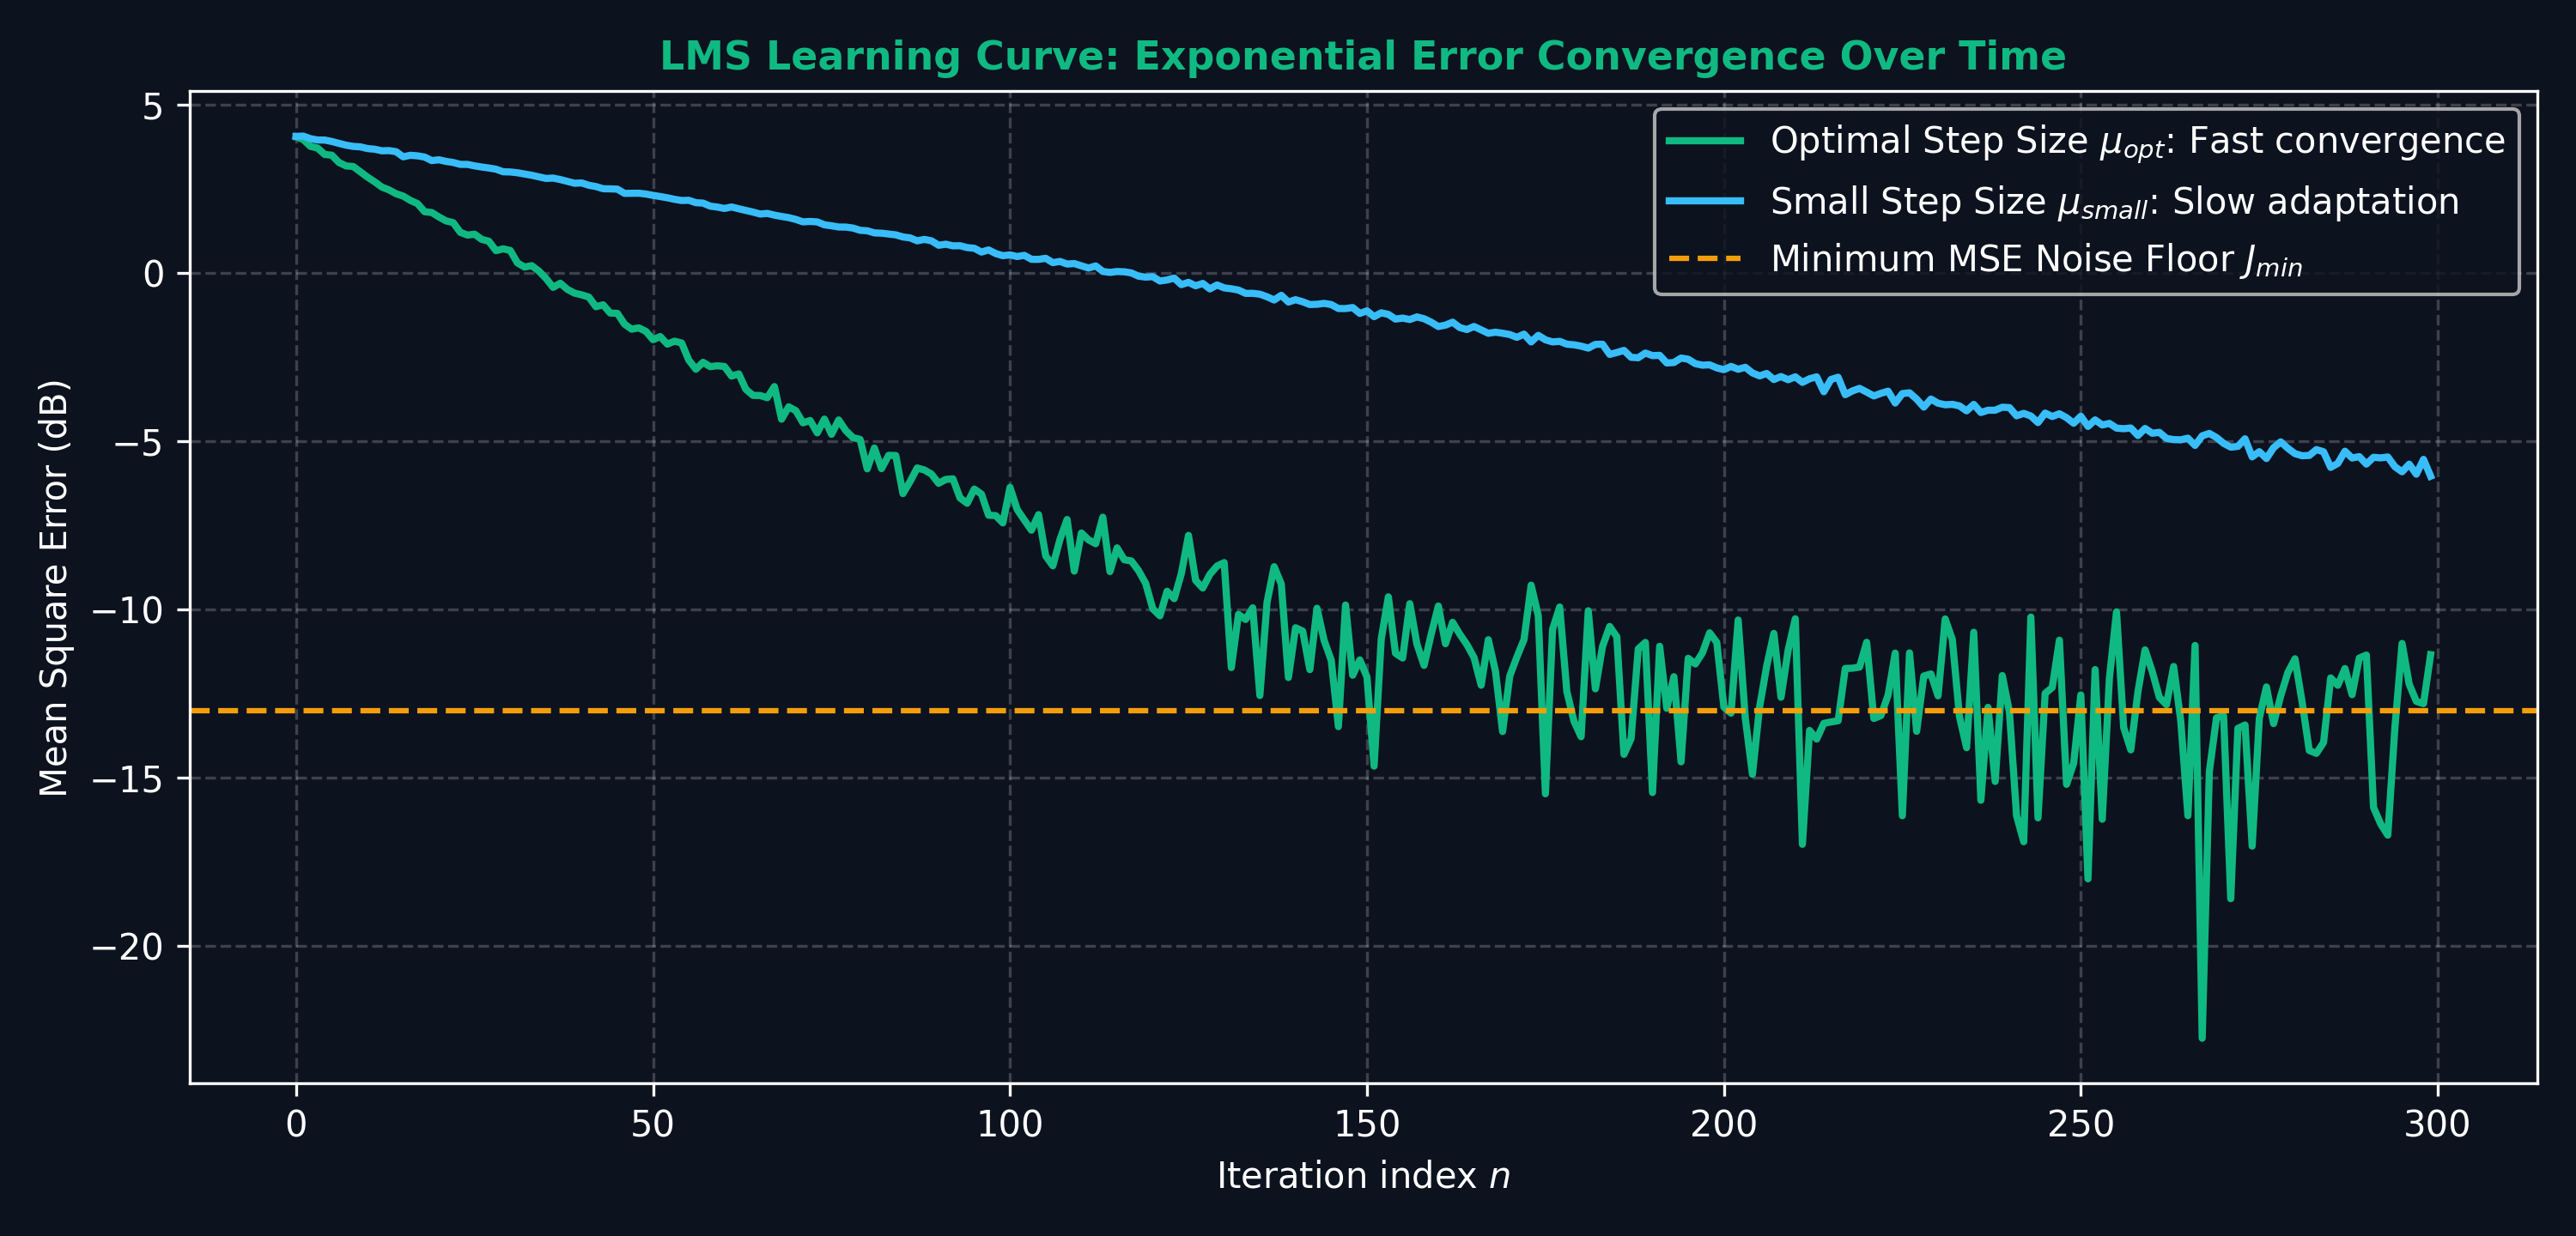
\includegraphics[width=0.85\textwidth]{images/lms_learning_curve_weights.png}
    \caption{LMS Learning Curve: Exponential Error Convergence toward Theoretical Minimum MSE Floor.}
\end{figure}


Let the input vector be $\mathbf{x}(n) = [x[n], x[n-1], \dots, x[n-N+1]]^T$ and the weights be $\mathbf{w} = [w_0, w_1, \dots, w_{N-1}]^T$. 
The error is:
\begin{equation}
e[n] = d[n] - \mathbf{w}^T \mathbf{x}(n)
\end{equation}
We minimize the Mean Squared Error (MSE):
\begin{equation}
J(\mathbf{w}) = E[e^2[n]] = E[d^2[n]] - 2\mathbf{w}^T \mathbf{r} + \mathbf{w}^T \mathbf{R} \mathbf{w}
\end{equation}
where $\mathbf{R} = E[\mathbf{x}(n)\mathbf{x}^T(n)]$ and $\mathbf{r} = E[d[n]\mathbf{x}(n)]$.
The minimum MSE is $\xi_{min} = J(\mathbf{w}_{opt})$ where $\mathbf{w}_{opt} = \mathbf{R}^{-1}\mathbf{r}$. We can rewrite $J(\mathbf{w})$ as:
\begin{equation}
J(\mathbf{w}) = \xi_{min} + (\mathbf{w} - \mathbf{w}_{opt})^T \mathbf{R} (\mathbf{w} - \mathbf{w}_{opt})
\end{equation}
The gradient is:
\begin{equation}
\nabla J = 2\mathbf{R}\mathbf{w} - 2\mathbf{r}
\end{equation}
The steepest descent update rule is:
\begin{equation}
\mathbf{w}(n+1) = \mathbf{w}(n) - \mu \nabla J = \mathbf{w}(n) + 2\mu (\mathbf{r} - \mathbf{R}\mathbf{w}(n))
\end{equation}
For stability, step size $\mu$ must satisfy:
\begin{equation}
0 < \mu < \frac{1}{\lambda_{max}}
\end{equation}

\section{LMS Algorithm Derivation}
Since we don't know $\mathbf{R}$ and $\mathbf{r}$, we use the instantaneous gradient:
\begin{equation}
\hat{\nabla} J \approx -2e[n]\mathbf{x}(n)
\end{equation}
Substituting this into the update rule gives the \textbf{LMS Algorithm}:
\begin{equation}
\mathbf{w}(n+1) = \mathbf{w}(n) + 2\mu e[n]\mathbf{x}(n)
\end{equation}
The convergence condition in practice is:
\begin{equation}
0 < \mu < \frac{1}{\text{tr}(\mathbf{R})} = \frac{1}{N P_x}
\end{equation}
The time constant for the $k$-th mode is $\tau_k \approx \frac{1}{4\mu\lambda_k}$.

\section{Misadjustment and NLMS}
The excess MSE due to gradient noise causes \textbf{Misadjustment} $M$:
\begin{equation}
M = \frac{\mu \text{tr}(\mathbf{R})}{1 - \mu\text{tr}(\mathbf{R})} \approx \mu N P_x
\end{equation}
There is a trade-off: large $\mu$ yields fast convergence but high misadjustment.

To handle varying input power, the \textbf{Normalized LMS (NLMS)} adjusts $\mu$ dynamically:
\begin{equation}
\mu(n) = \frac{\alpha}{\epsilon + \|\mathbf{x}(n)\|^2}
\end{equation}
\begin{equation}
\mathbf{w}(n+1) = \mathbf{w}(n) + \frac{2\alpha}{\epsilon + \|\mathbf{x}(n)\|^2} e[n]\mathbf{x}(n)
\end{equation}

\section{Recursive Least Squares (RLS)}
RLS minimizes a deterministically weighted sum of squared errors with a forgetting factor $\lambda$:
\begin{equation}
\mathcal{E}(n) = \sum_{i=1}^n \lambda^{n-i} e^2[i]
\end{equation}
It uses the Matrix Inversion Lemma to update $P(n) = \mathbf{R}^{-1}(n)$:
\begin{equation}
P(n) = \lambda^{-1}[P(n-1) - \mathbf{k}(n)\mathbf{x}^T(n)P(n-1)]
\end{equation}
RLS has $O(N^2)$ complexity but much faster convergence.

\section{Applications}
Adaptive filters are used in acoustic echo cancellation, adaptive noise cancellation, channel equalization, and beamforming. 


\section{Key Formulas}
\begin{table}[H]
\centering
\begin{tabular}{ll}
\toprule
\textbf{Concept} & \textbf{Formula} \\
\midrule
MSE Cost Function & $J(\mathbf{w}) = \xi_{min} + (\mathbf{w} - \mathbf{w}_{opt})^T \mathbf{R} (\mathbf{w} - \mathbf{w}_{opt})$ \\
Wiener Solution & $\mathbf{w}_{opt} = \mathbf{R}^{-1}\mathbf{r}$ \\
LMS Update Rule & $\mathbf{w}(n+1) = \mathbf{w}(n) + 2\mu e[n]\mathbf{x}(n)$ \\
Convergence Bound & $0 < \mu < \frac{1}{N P_x}$ \\
Misadjustment & $M \approx \mu N P_x$ \\
NLMS Update & $\mathbf{w}(n+1) = \mathbf{w}(n) + \frac{2\alpha}{\epsilon + \|\mathbf{x}(n)\|^2} e[n]\mathbf{x}(n)$ \\
\bottomrule
\end{tabular}
\end{table}

\section{Checkpoints}
\begin{itemize}
    \item \textbf{Q1:} An LMS filter has length $N=10$, input power $P_x=0.5$W. Calculate max $\mu$. 
    \newline \textit{Answer:} $\text{tr}(\mathbf{R}) = 10 \times 0.5 = 5$. Thus $\mu < 1/5 = 0.2$.
    \item \textbf{Q2:} Let $\mathbf{w}(0) = [0, 0]^T$, $\mu=0.1$, $\mathbf{x}(0) = [1, -2]^T$, $d[0]=2$. Find $\mathbf{w}(1)$.
    \newline \textit{Answer:} $y[0] = 0$, $e[0] = 2$. $\mathbf{w}(1) = [0, 0]^T + 2(0.1)(2)[1, -2]^T = [0.4, -0.8]^T$.
    \item \textbf{Q3:} If $\mu$ is halved from $0.01$ to $0.005$ with $N=20, P_x=1$, what is the new $M$?
    \newline \textit{Answer:} $M \approx \mu N P_x = 0.005 \times 20 \times 1 = 0.1$. The convergence time $\tau$ doubles.
\end{itemize}

\end{document}
